\documentclass[10pt, tikz]{standalone}
\usetikzlibrary{arrows}

\begin{document}
	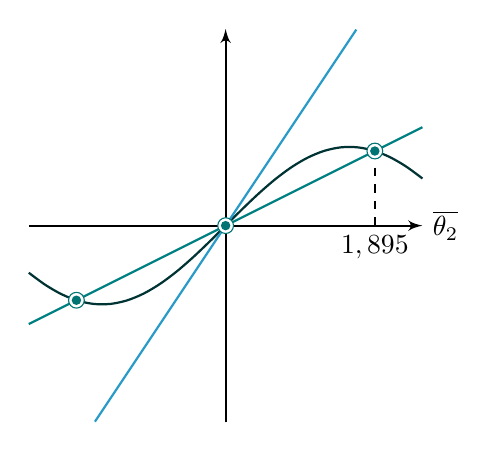
\begin{tikzpicture}[thick, scale=1]
		% eixos
		\draw [-latex'] (-2.5, 0) -- (2.5,0) node [right] {$\overline{\theta_2}$};
		\draw [-latex'] (0, -2.5) -- (0, 2.5);
		\draw [dashed] (1.895, 1.895/2) -- (1.895, 0) node [below] {$1,895$};
		
		% seno
		\draw [teal!40!black] 
			plot [smooth, variable=\x, domain=-2.5:2.5] ({\x}, {sin(\x*180/3.1415)})
		;
		
		% 0,5x
		\draw [teal]
			plot [variable=\x, domain=-2.5:2.5] ({\x}, {\x*0.5})
		;
		
		% 1,5x
		\draw [cyan!80!black]
			plot [variable=\x, domain=-1.66:1.66] ({\x}, {\x*1.5})
		;
		
		% intersecções
		\draw [thin, teal!90!black, fill=white]
			(0,0) circle (0.1)
		;
		\fill [teal!90!black]
			(0,0) circle (0.06)
		;
		\draw [thin, teal!90!black, fill=white]
			(1.895, 1.895/2) circle (0.1)
		;
		\fill [teal!90!black]
			(1.895, 1.895/2) circle (0.06)
		;
		\draw [thin, teal!90!black, fill=white]
			(-1.895,-1.895/2) circle (0.1)
		;
		\fill [teal!90!black]
			(-1.895,-1.895/2) circle (0.06)
		;
	\end{tikzpicture}
\end{document}